\begin{figure}
    \begin{center}
    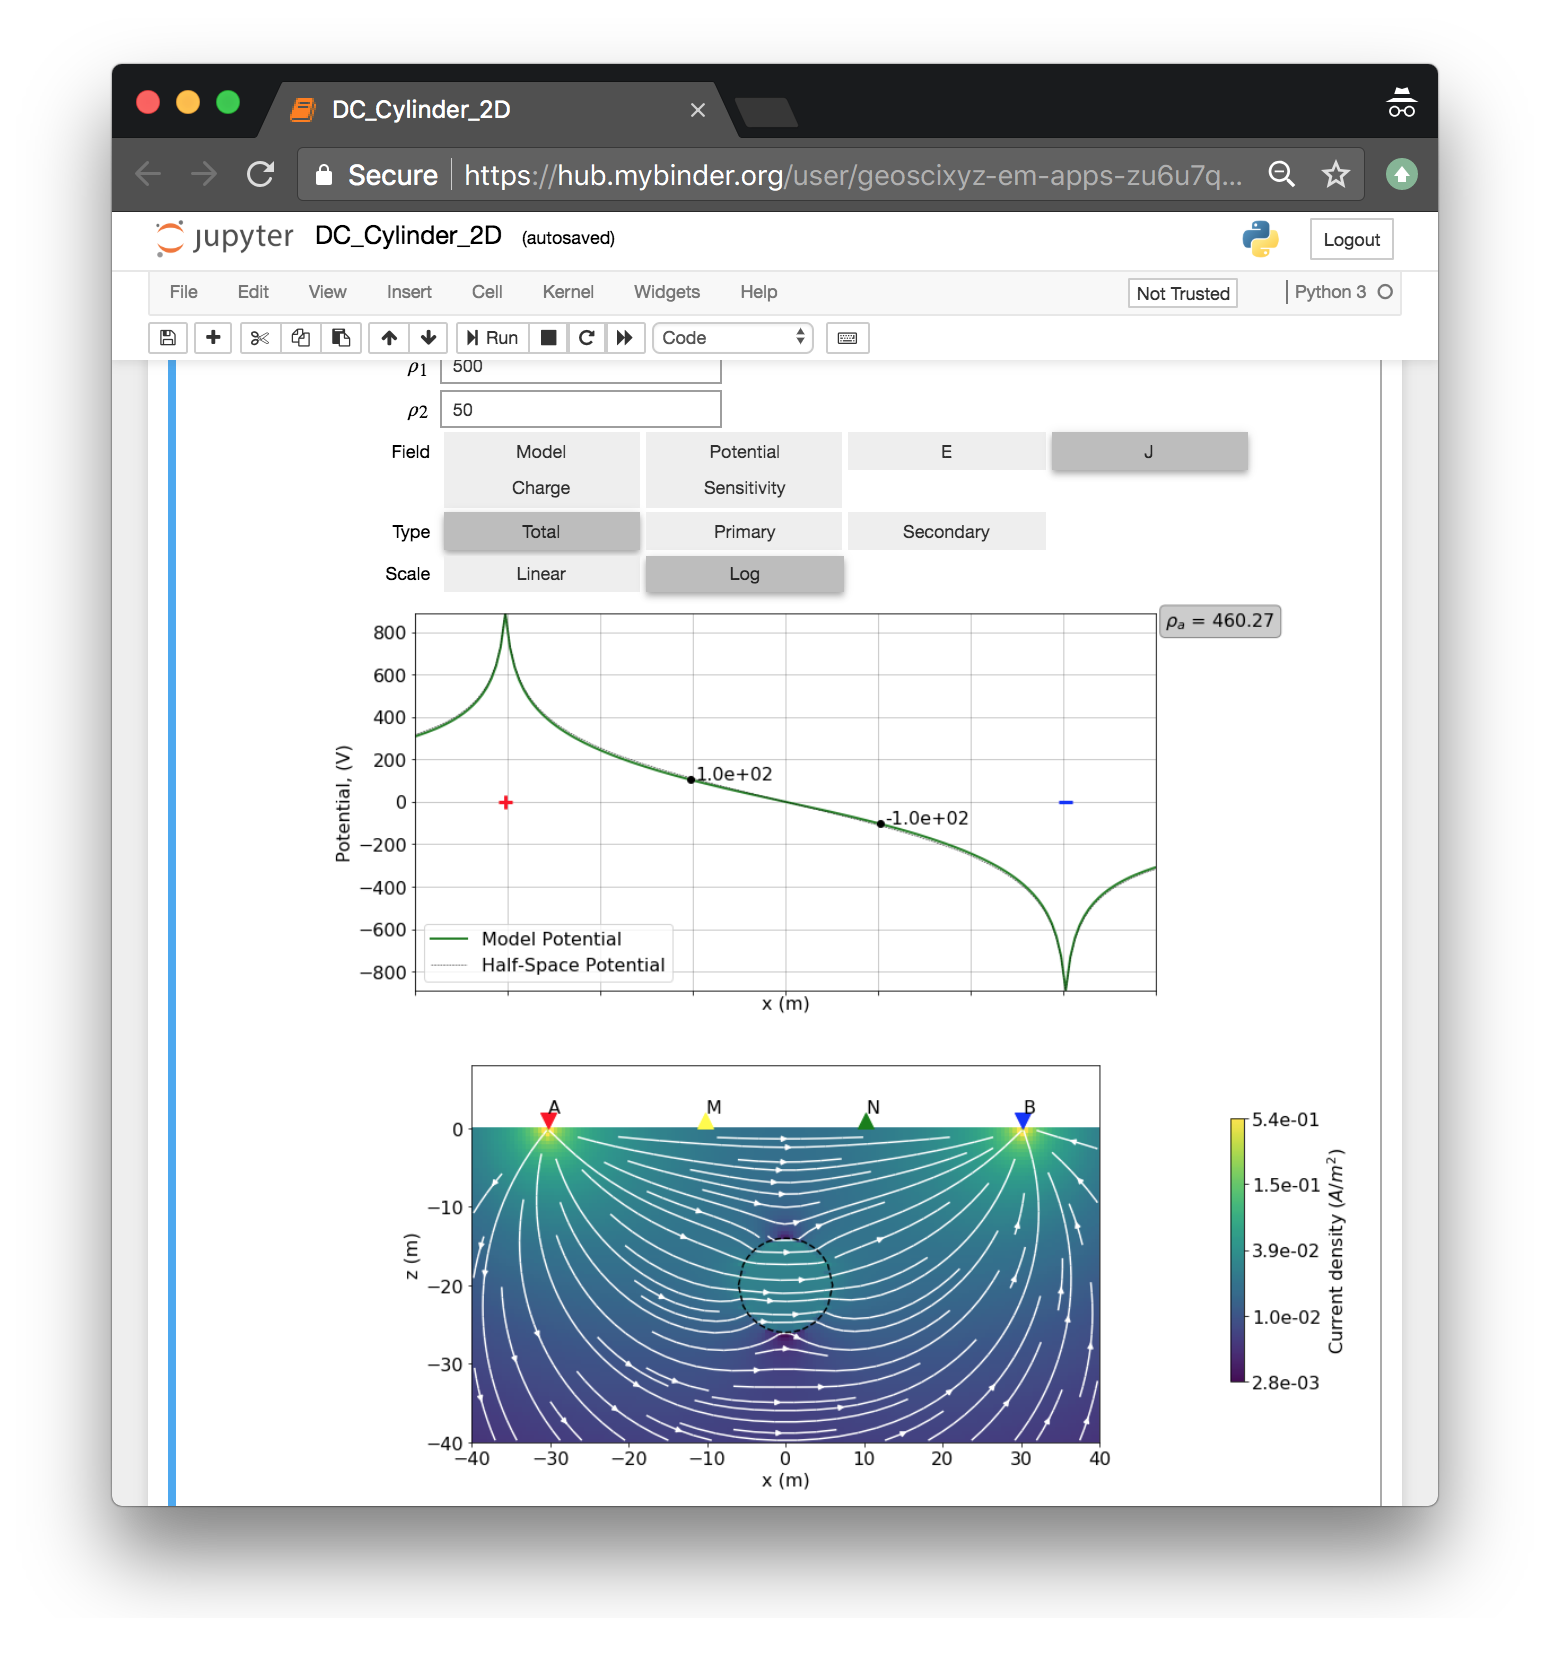
\includegraphics[width=\textwidth]{figures/education/jupyter-app.png}
    \end{center}
\caption{
   A sample Jupyter notebook ``app'' that simulates a DC resistivity over a halfspace
   with a cylinder. The widgets control the visualization. The user can change the model parameters
   (e.g. the resistivity of the cylinder and of the background), the survey geometry, and select the visualization
   (e.g. electric field, currents, charges, etc.)
}
\label{fig:jupyter-app}
\end{figure}



